\documentclass[tikz]{standalone}
\usetikzlibrary{trees}
\tikzstyle{treenode} = [draw=black,thick,anchor=west]
\begin{document}
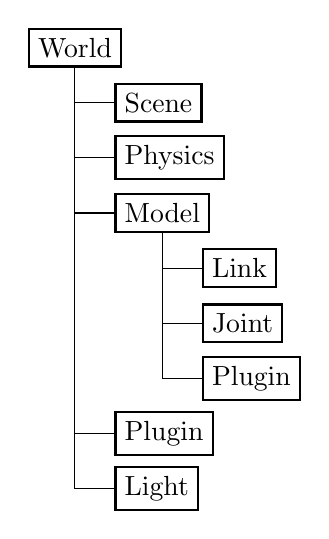
\begin{tikzpicture}[%
    grow via three points={one child at (0.5,-0.7) and two children at (0.5,-0.7) and (0.5,-1.4)},
    edge from parent path={(\tikzparentnode.south) |- (\tikzchildnode.west)}]
  \node[treenode]  {World}
  child { node[treenode] {Scene} }
  child { node[treenode] {Physics} }
  child { node[treenode] {Model}
      child { node[treenode] {Link} }
      child { node[treenode] {Joint} }
      child { node[treenode] {Plugin} }
    }
  child [missing] {}
  child [missing] {}
  child [missing] {}
  child { node[treenode] {Plugin} }
  child { node[treenode] {Light} };
\end{tikzpicture}
\end{document}
